\documentclass[11pt]{article}

% Load packages
\usepackage{amsthm,amsmath,amssymb}
\usepackage{dsfont}
\usepackage{graphicx}
\usepackage{natbib}
\usepackage[colorlinks,citecolor=blue,urlcolor=blue]{hyperref}
\usepackage[utf8]{inputenc}
\usepackage[margin = 2.5cm]{geometry}
\usepackage{booktabs}
\usepackage{float}

\usepackage{tikz}
\usetikzlibrary{shapes,decorations,arrows,calc,arrows.meta,fit,positioning}
\tikzset{
	-Latex,auto,node distance =1 cm and 1 cm,semithick,
	state/.style ={ellipse, draw, minimum width = 0.7 cm},
	point/.style = {circle, draw, inner sep=0.04cm,fill,node contents={}},
	bidirected/.style={Latex-Latex,dashed},
	el/.style = {inner sep=2pt, align=left, sloped}
}

\usepackage{sectsty}
\sectionfont{\fontsize{12}{16}\selectfont\centering}
\subsectionfont{\fontsize{11}{14}\selectfont}

\usepackage{hyperref}
\hypersetup{colorlinks,linkcolor={blue},citecolor={blue},urlcolor={blue}}  

% define helper commands
\newcommand{\E}{\mathbb{E}}
\newcommand{\Prob}{\mathbb{P}}


% Title Page
\title{The Impact of Natural Disasters on Education: \\ Evidence from Standardized Testing}
\author{Gregor Steiner}


\begin{document}
\maketitle

\begin{abstract}
	\centering
	\begin{minipage}{\dimexpr\paperwidth-10cm}
		Few studies have investigated the impact of natural disasters on academic performance. We use an event-study design to estimate dynamic treatment effects of natural disasters on students' performance in standardized tests. We find a significant effect on the performance in mathematics in the period of the disaster. For the performance in Reading Language Arts we find no significant effect.
	\end{minipage}
\end{abstract}


% sections

\section{Introduction}

Natural disasters are responsible for massive economic damage and due to climate change the frequency of such disasters will increase in most regions \citep{IPCC_2021}. Therefore, it is essential to have a good understanding of the consequences. While much research has been done on the macroeconomic consequences of natural disasters, few studies have focused on the impact on education. This study investigates the effect of natural disasters on academic performance.

A causal effect of natural disasters may be driven by school closures \citep{Grewening_2020}, destroyed infrastructure, and emotional stress \citep{Vogel_2016}. Furthermore, some forms of natural disasters, e.g. extreme heat, may directly impair cognitive performance \citep{Ramsey_1995}.

To identify dynamic causal effects of experiencing natural disasters, this paper uses an event-study design. In particular, we estimate dynamic treatment effects for up to eight years after initial treatment. As a result, not only short-term but also medium to long-term effects can be found. Since treatment effects are likely very heterogenous, we use the estimator by \cite{Sun_2021}. 

This article uses standardized test data on a US county level for grades 3 through 8 in mathematics and reading language arts (RLA) to measure academic performance, covering the school years 2008/2009 to 2018/2019. This measure is very attractive as the test scores are standardized relative to a national reference cohort. Therefore, the outcomes are nationally comparable. For the same period, we obtain data on natural disasters from declarations by the Federal Emergency Management Agency and data on storms from the National Weather Service.

This article contributes to a rich literature on economic effects of natural disasters. More specifically, this paper contributes to the literature on the impact of natural disasters on education. Previous work has produced mixed results. Some authors find significant effects of natural disasters on the education system \citep{Holmes_2002, Cuaresma_2010, Sacerdote_2012, Goodman_2020}, while others find no or only small effects \citep{Baggerly_2008, Pane_2008}. Morover, some authors find large differences by subject \citep{Spencer_2016}.

Previous studies have concentrated on a single type, or even a single instance of disasters. For example, hurricane Katrina has been the subject of many studies \citep[e.g.][]{Sacerdote_2012, Deryugina_2018}. To the best of our knowledge, this is the first study to exploit a very comprehensive dataset of natural disasters, including various different types of disasters. 

The rest of this paper is organized as follows: Section \ref{Data} introduces the data used and presents some descriptive statistics. Section \ref{EmpStrat} explains the empirical strategy. Section \ref{Results} discusses the results and section \ref{Conclusion} concludes.




\section{Data}

\subsection{Natural Disaster Data}

Natural disasters are declared as such by the president, usually upon request by the affected state's governor. Once a disaster is federally declared, states or local governments can receive federal assistance. The Federal Emergency Management Agency (FEMA) provides data on all federally declared natural disasters, beginning in 1953. The data is easily accessible via their API \citep{rfema}.

Figure \ref{DisasterMap} shows the number of declared disasters since 1953 across the US. It seems that the variation in the number of declared disasters may be driven by the governor's proactiveness in requesting a declaration. Thus, it could be interesting to compare counties on different sides of state borders, whose actual disaster exposure is likely very similar in order to analyze the effect of a declaration.



\begin{figure}[!h]
	\centering
	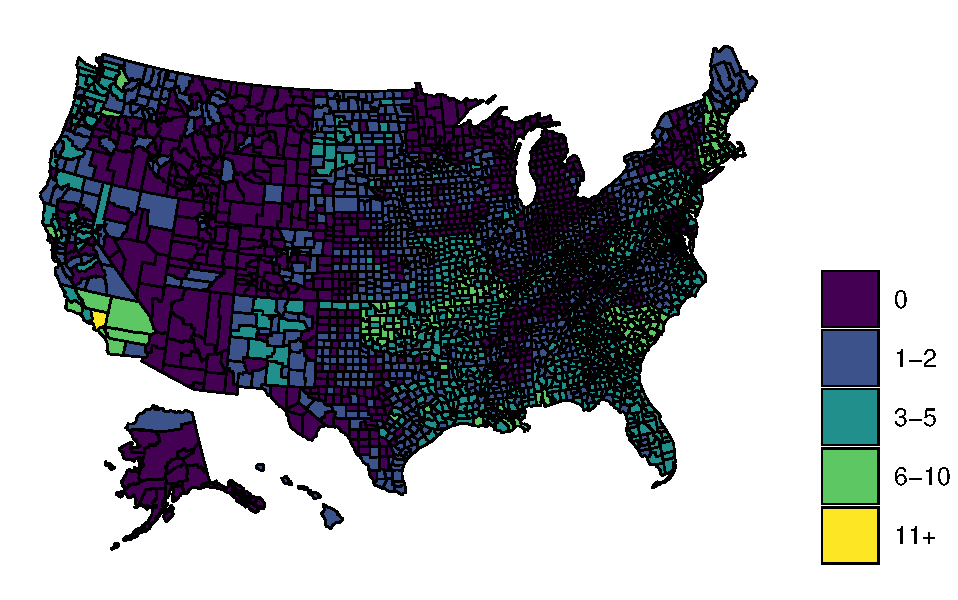
\includegraphics[scale=0.7]{"../Code & Data/DisasterMap.png"}
	\caption{Number of declared natural disasters from 2008 to 2018}
	\label{DisasterMap}
\end{figure}


FEMA also provides federal disaster assistance data. This includes the amount of damage caused and amount of federal disaster assistance granted. Unfortunately, this data is only available since October 2016. Figure \ref{AssistanceMap} shows the total federal assistance awarded to counties.


\begin{figure}[!h]
	\centering
	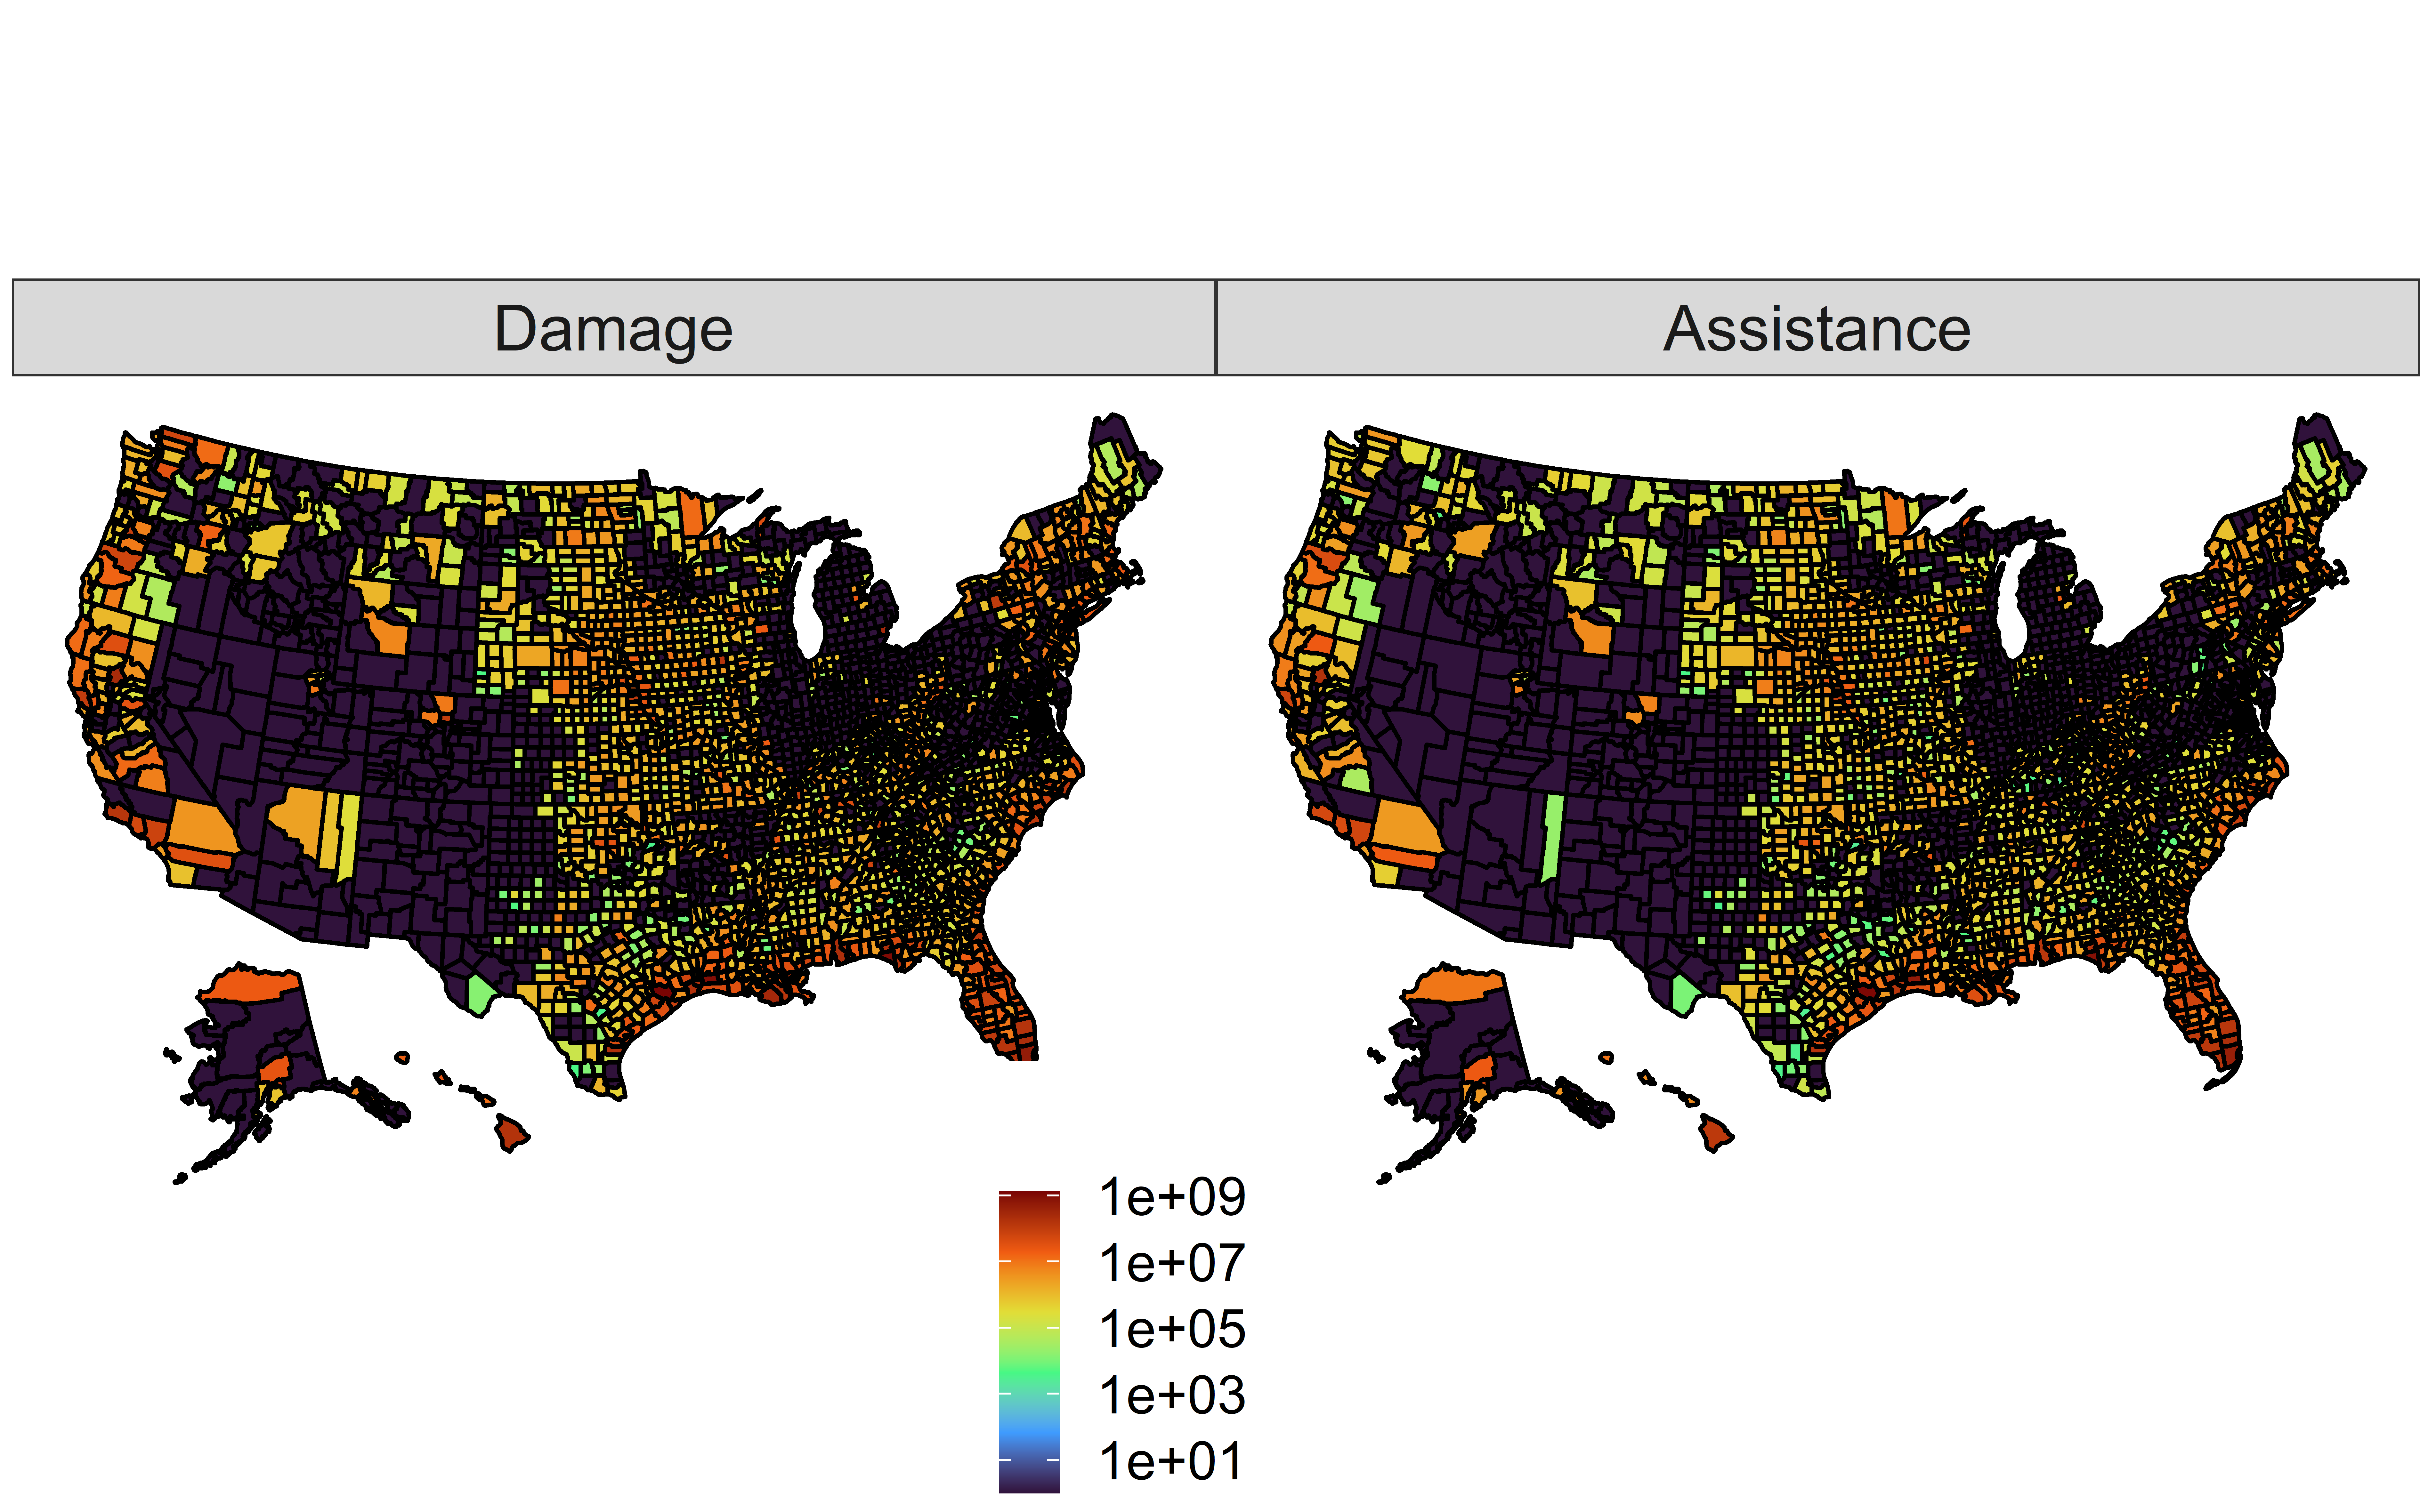
\includegraphics[scale=0.7]{"../Code & Data/AssistanceMap.png"}
	\caption{Amount of federal disaster assistance (in USD) awarded to counties since October 2016}
	\label{AssistanceMap}
\end{figure}




\subsection{Standardized Testing Data}

Data on academic achievement is available from the Stanford Education Data Archive \citep{SEDA}. They provide mean test results from standardized tests by county, year, grade and subject among all students and various subgroups (including race, gender, and economically disadvantaged). The most recent version 4.1 covers grades 3 through 8 in mathematics and Reading Language Arts (RLA) over the 2008-09 through 2017-18 school years.

Test scores are cohort-standardized, meaning they can be interpreted relatively to an average national reference cohort in the same grade. For instance, a county mean of 0.5 indicates that the average student in the county scored approximately one half of a standard deviation higher than the average national student in the same grade.

In addition to mean test scores, the data includes estimates of gap estimates for various subgroups, e.g. mean difference in test scores among white and black students. These are only reported if the subgroups' sample sizes are large enough. Thus, the number of observations for some of the gap statistics is substantially smaller.

Furthermore, the Stanford Education Data Archive maintains a large set of covariates for each county and year. They include variables like the county's median income, unemployment and ethnic proportions.


\subsection{Combining disaster and testing data}

Natural disasters should only have an effect on test scores if they occur before the test. Standardized tests are generally administered during spring. We will use March 1st as a cut-off point. Thus, any disaster happening within the same school year before the 1st of March will be considered. School years tend to start in late August or early September with some variation across states. We will use September 1st, meaning any disaster happening between September 1st and March 1st will be counted for a given school year.

Each disaster is assigned to a school year as described above. Then, disaster and test score data can be merged by school year and county. This yields a panel data set with six grades and two subjects for each county-year combination. Table \ref{SumStats} shows summary statistics for all relevant variables

\begin{table}[!htbp] \centering \renewcommand*{\arraystretch}{1.1}\caption{Summary Statistics}\label{SumStats}\resizebox{\textwidth}{!}{
\begin{tabular}{lrrrrrrr}
\hline
\hline
Variable & N & Mean & Std. Dev. & Min & Pctl. 25 & Pctl. 75 & Max \\ 
\hline
Disasters & 331778 & 0.222 & 0.569 & 0 & 0 & 0 & 6 \\ 
Disaster Dummy & 331778 &  &  &  &  &  &  \\ 
... 0 & 278656 & 84\% &  &  &  &  &  \\ 
... 1 & 53122 & 16\% &  &  &  &  &  \\ 
Cumulative Disasters & 331778 & 1.259 & 1.645 & 0 & 0 & 2 & 14 \\ 
Grade & 339264 &  &  &  &  &  &  \\ 
... 3 & 58762 & 17.3\% &  &  &  &  &  \\ 
... 4 & 58660 & 17.3\% &  &  &  &  &  \\ 
... 5 & 57417 & 16.9\% &  &  &  &  &  \\ 
... 6 & 57146 & 16.8\% &  &  &  &  &  \\ 
... 7 & 54538 & 16.1\% &  &  &  &  &  \\ 
... 8 & 52741 & 15.5\% &  &  &  &  &  \\ 
Subject & 339264 &  &  &  &  &  &  \\ 
... Mathematics & 165780 & 48.9\% &  &  &  &  &  \\ 
... RLA & 173484 & 51.1\% &  &  &  &  &  \\ 
Mean test score & 328273 & -0.041 & 0.294 & -3.196 & -0.214 & 0.152 & 1.669 \\ 
White-Black gap & 131047 & 0.618 & 0.256 & -0.754 & 0.454 & 0.771 & 2.358 \\ 
Male-Female gap & 306961 & -0.131 & 0.199 & -1.612 & -0.258 & 0.001 & 1.248 \\ 
Disadvantaged gap & 283272 & 0.543 & 0.211 & -0.995 & 0.413 & 0.669 & 2.052 \\ 
Log Income & 339003 & 10.693 & 0.253 & 9.305 & 10.547 & 10.835 & 11.727 \\ 
Unemployment & 339003 & 0.078 & 0.032 & 0.001 & 0.057 & 0.096 & 0.3\\ 
\hline
\hline
\end{tabular}
}
\end{table}













\section{Empirical Strategy}

\subsection{Setting}

We employ an event study design to measure the effect of natural disasters on standardized test outcomes. An event study design is a staggered adoption design where units are first-treated at different points in time, and there may or may not be never-treated units \citep{Sun_2021}.

In order to identify a causal effect, unobservable determinants of a county's test scores must be unrelated to natural disasters conditional on observable characteristics of that county. The occurrence of natural disasters is plausibly random conditional on location. Furthermore conditioning on the year should account for an increasing trend in natural disasters due to climate change. Thus, independence of mean test scores and natural disasters is plausible conditional on county and year fixed effects.

Consequently, the baseline specification is
\begin{align} \label{baseline}
	y_{i, t, g} = \sum_{l = -9, l \neq -1}^{8} \beta_l D_{i, t-l} + \alpha_i + \lambda_t + \zeta_g + X_{i, t} \gamma + \varepsilon_{i, t, g} \;,
\end{align}
where $y_{i, t, g}$ is the outcome of interest for county $i$, year $t$, and grade $g$. County, year, and grade fixed-effects are given by $\alpha_i$, $\lambda_t$, and $\zeta_g$ respectively and $X_{i, t}$ is a row vector of additional control variables. $D_{i, t-l}$ is a treatment indicator for county $i$ in year $t-l$. That is, $D_{i, t-l} = 1$ if the county had already experienced a disaster $l$ years ago at time $t$.

Since we consider the time period 2009-2018, $-9 \leq l \leq 9$, but note that $l = 9$ would correspond to a unit that experienced a disaster in the first period and is therefore always treated. As recommended by \cite{Sun_2021}, these units are dropped from estimation, since no treatment effects can be identified for that group\footnote{At least not under standard assumptions. If one is willing to make assumptions about the trends of both potential outcomes, then it may make sense to keep always treated units \citep[see][]{Marcus_2021}, but this is not the case here.}.

Also, we need to drop at least two leads or lags to avoid a multicollinearity problem. A complete set of treatment leads and lags is perfectly collinear with unit and time fixed-effects \citep[for an extensive discussion of this issue see][section 3.2]{Borusyak_2021}. It is common to drop the first relative indicator prior to treatment (i.e. $\beta_{-1} = 0$). This acts as a normalization of treatment relative to the period before treatment. Furthermore, we bin the distant leads, that is we combine the treatment indicators for $l \leq -5$. Thus, equation (\ref{baseline}) turns into
\begin{align} \label{baselineBinned}
	y_{i, t, g} = \beta_{-5} \sum_{l \leq -5} D_{i, t-l} + \sum_{l = -4, l \neq -1}^{8} \beta_l D_{i, t-l} + \alpha_i + \lambda_t + \zeta_g + X_{i, t} \gamma + \varepsilon_{i, t, g} \;.
\end{align}
Note that treatment must be absorbing, meaning the sequence $(D_{i, t})_{t=1}^T$ must be a non-decreasing sequence of $0$s and $1$s. In other words, after being treated for the first time a county stays treated. In the present application this means treatment refers to having experienced a disaster rather than experiencing a disaster in that year. This is common practice and does not cause bias due to the conditionally random nature of natural disasters \citep{Deryugina_2017}. Thus, the emphasis lies on cumulative long-term effects rather than instantaneous short-term effects.

It is implausible that the treatment effects are constant in our setting. The extent of disasters varies substantially, and also the level of preparation for such disasters likely displays high variance across counties. 

\subsection{Interaction-weighted estimator}

We utilize the interaction-weighted (IW) estimator proposed by \cite{Sun_2021} that is robust to treatment effects heterogeneity. The main interest lies on the cohort average treatment effect on the treated (CATT),
\begin{align*}
	CATT_{e, l} := \E \left[ Y_{i, t+l} - Y_{i, t+l}^{\infty} | E_i = e \right],
\end{align*}
where $Y_{i, t+l}^{\infty}$ is the counterfactual of being never treated and $E_i$ denotes the first treatment period. Thus, $CATT_{e, l}$ is the average treatment effect on the treated $l$ years after being treated for the first time for the cohort that was first treated in year $e$.

The estimation procedure consists of three main steps:
\begin{enumerate}
	\item Estimate $CATT_{e, l}$ using a linear fixed effects specification with interactions between relative period indicators and cohort indicators:
	\begin{align} \label{CATTDID}
		y_{i, t, g} = \sum_{e \notin C}^{}\sum_{l \neq -1}^{} \delta_{e, l} (\mathds{1}\{E_i = e\} D_{i, t-l}) + \alpha_i + \lambda_t + \zeta_g + \varepsilon_{i, t, g} \;,
	\end{align}
	where $C$ is the set of comparison cohorts. In our case $C$ is the never treated cohort, i.e. $C = {\infty}$. If there is a cohort that is always treated, i.e. that already receives treatment in the first period, then we need to exclude this cohort. The coeffiecient estimator $\widehat{\delta}_{e, l}$ that we obtain from (\ref{CATTDID}) estimates $CATT_{e, l}$.
	
	\item Weight the estimators by the share of the respective cohort in the sample in that period. Let $\hat{W}^l$ be a weight matrix with element $(t, e)$
	\begin{align*}
		[\widehat{W}^l]_{t, e} := \frac{\mathds{1}\{t - e = l\} \sum_{i = 1}^{N} \mathds{1}\{E_i = e\}}{\sum_{e \in h^{l}} \sum_{i = 1}^{N} \mathds{1}\{E_i = e\}},
	\end{align*}
	where $h^{l} := \{e: 1 - l \leq e \leq \max(E_i) - 1 - l\}$ is the set of cohorts that experience at least $l$ periods of treatment.
	
	\item Take the average over all $CATT_{e, l}$ estimates weighted by the cohort shares in the weight matrices. Let $vec(A)$ be the vectorize operator that vectorizes matrix $A$ by stacking its columns and let $\widehat{\delta}$ be the vector that collects $\widehat{\delta}_{e, l}$ for all $e$ and $l$. Then, the IW estimator $\widehat{v}_g$ for bin $g$ can be written as 
	\begin{align}
		\widehat{v}_g := \frac{1}{|g|} \sum_{l \in g} [vec(\widehat{W}^l)]^\intercal \widehat{\delta}.
	\end{align}
	For a singleton bin $g = \{l\}$, this simplifies to
	\begin{align*}
		\widehat{v}_{g} := [vec(\widehat{W}^l)]^\intercal \widehat{\delta}.
	\end{align*}
	
\end{enumerate}

Under some standard assumptions, $\widehat{v}_g$ is asymptotically normal \citep[for a proof and a detailed description of said assumptions see][Appendix C]{Sun_2021}. Under the additional assumptions of parallel trends and no anticipatory behavior, $\widehat{v}_g$ is consistent, that is it converges in probability to
\begin{align*}
	\widehat{v}_g \overset{p}{\to} [vec(W^{l})]^\intercal \delta = \sum_{e \in h^{l}} \Prob(E_i = e | E_i \in h^{l}) CATT_{e, l} \; ,
\end{align*}
where $W^{l}$ is the probability limit of the weight matrix $\widehat{W}^l$.


We use the existing implementation in the \textbf{fixest} R package \citep{Berge_2018}.

\subsection{Identifying assumptions}

Below we discuss the identifying assumptions.

\textbf{Parallel Trends:} Parallel trends in the sense of \cite{Sun_2021} refers to the following: $\E[Y_{i, t}^{\infty} - Y_{i, s}^{\infty} | E_i = e]$ does not depend on $e$ for any $s \neq t$. That is, the expected temporal difference, i.e. the trend, in the potential outcomes of being never-treated is the same for all treatment timings. A conditional version of the assumption, as in \cite{Callaway_2021}, should definitely hold, as test scores and natural disasters are plausibly independent given location. However, we cannot be sure about the unconditional version.

Testing for parallel trends is problematic for two reasons: These tests tend to have very low power and they introduce selective inference type issues if inference is conditional on passing a parallel trends test \citep{Rambachan_2019}.

\textbf{No Anticipatory Behavior:} There is no treatment effect prior to treatment, that is $\E[Y_{i, e+l} - Y_{i, e+l}^{\infty}] = 0$ for all $e$ and all $l < 0$. This assumption is plausible as the treatment path is not known. Natural disasters are quasi-random and cannot be reliably forecast more than a few days in advance.






\section{Results} \label{Results}

Figure \ref{ResultsPlot} shows estimated dynamic treatment effects and 95\% confidence intervals for all students and the four subgroups of interest. 

\begin{figure}[!h]
	\centering
	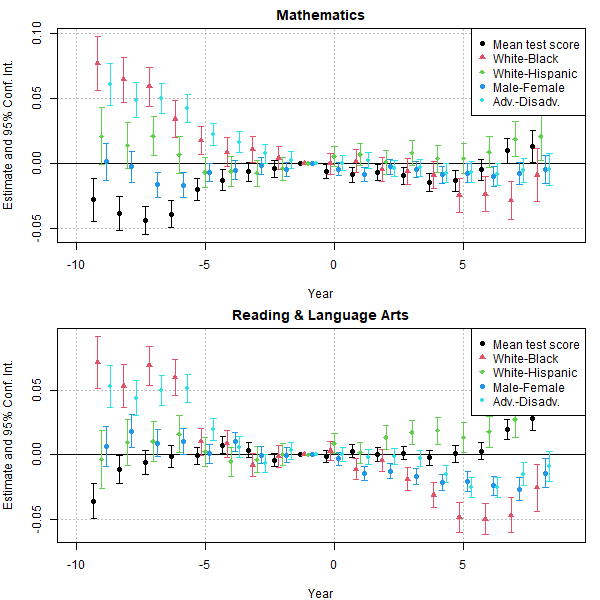
\includegraphics[scale=1]{"../Code & Data/ResultsPlot.pdf"}
	\caption{Dynamic Treatment effects in relative time: FEMA disaster data}
	\label{ResultsPlot}
\end{figure}


For the period of treatment there is a significant\footnote{Significant is used here in the sense that a confidence interval with nominal coverage of 95\% does not include zero, that is a corresponding t-test would reject the null hypothesis of a zero effect at the 5\% level.} effect of natural disasters on the performance in mathematics. The effect size is between just above zero and -0.01 standard deviations. Also, one year after the disaster there is an even larger significant decrease in test scores. For all subsequent periods the effect is not significant. There are some point estimates well below zero, but the uncertainty around those is relatively large. For performance in RLA, there are no significant effects.

Note that the number of observed units decreases with the distance in time from treatment. The reason for this is that in order to experience eight treated years, the county has to experience its first disaster very early. Similarly, it has to receive treatment very late to experience more than five years before treatment. As a result, the uncertainty increases with the distance in time from treatment.

For the subgroups we find some surprising results. Black students seem to perform better in RLA in the medium term after a disaster. That is, there are significantly positive results one to seven years after treatment. The effect sizes are substantial: Seven years after treatment the increase in RLA performance goes up to 0.1 standard deviations. In other words, the average black student sees an increase in performance of up to 0.1 standard deviations of the national reference cohort. Also, hispanic students score significantly lower in mathematics in the year following a disaster.



Positive effects of disasters on performance are not unheard of in the literature. In fact, this is somewhat consistent with the findings by \cite{Sacerdote_2012}. Many students have to switch schools and some may even benefit from attending a higher quality school after the disaster. Black students may disproportionally attend lower quality schools and are therefore more likely to benefit from having to switch schools. 

Figures \ref{ResultsPlotStorm} shows the same graphs based on the storm treatment. The results look very similar. In the period of the storm there is a significant decrease in mathematics scores of up to -0.015 standard deviations. For the years following treatment there are no significant effects.

For female students there is a significant decrease in both subjects in the period of the storm. For RLA we even find a significantly negative effect one year after the storm. Similarly, economically disadvantaged students perform worse in the period of treatment and in RLA one year after treatment. The effect sizes range from barely above zero up to -0.015 or even -0.02 standard deviations. For black and hispanic students we do not find any significant effects of the storm treatment.

\begin{figure}[!h]
	\centering
	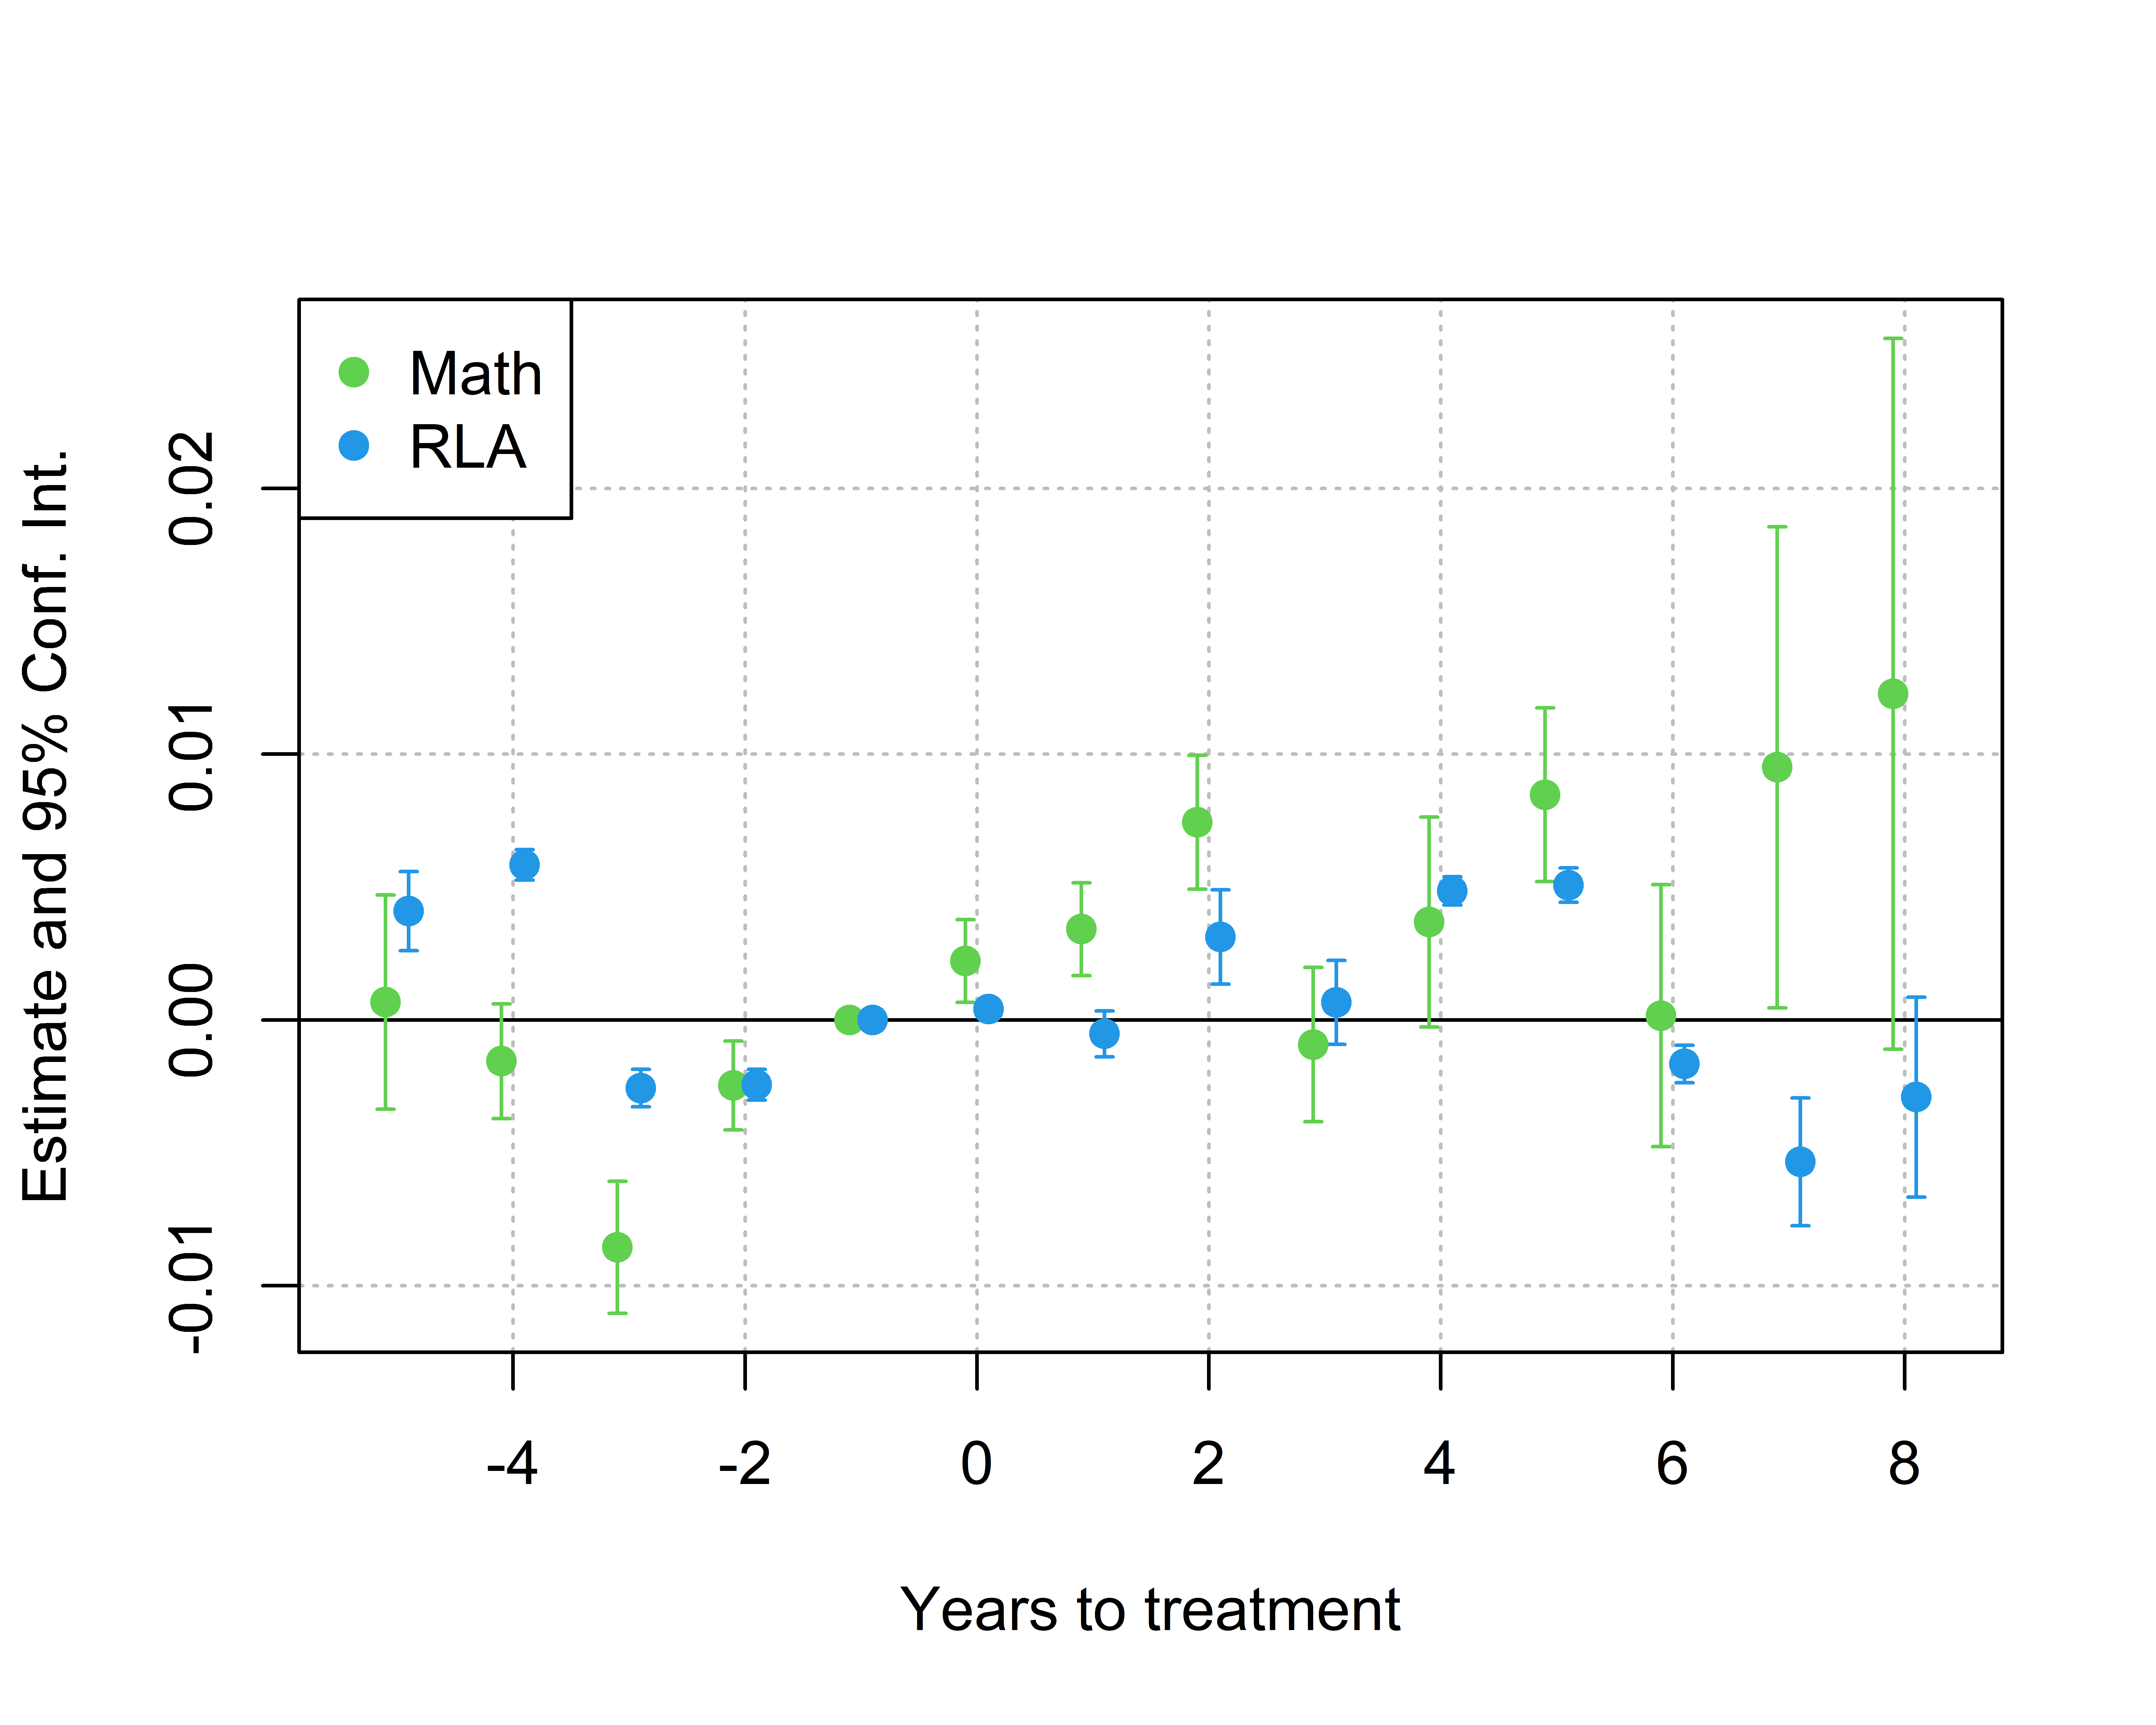
\includegraphics[scale=1]{"../Code & Data/ResultsPlotStorm.pdf"}
	\caption{Dynamic Treatment effects in relative time: NWS storm data}
	\label{ResultsPlotStorm}
\end{figure}


It could be the case that medium- and long-term effects are largely driven by migration. That's why it may be interesting to have a look at the ethnic composition of the counties relative to initial treatment. Figure \ref{EthnicComposition} shows ethnic shares for the treated counties in relative time.

\begin{figure}[!h]
	\centering
	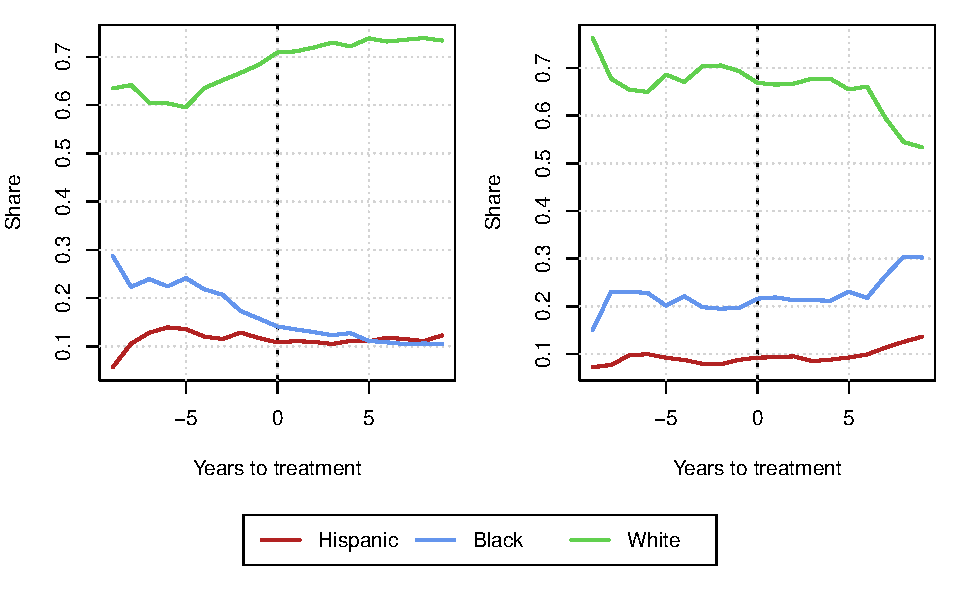
\includegraphics[scale=1]{"../Code & Data/EthnicComposition.pdf"}
	\caption{Aggregated ethnic shares by treatment timing based on FEMA disasters (left) and on NWS storms (right)}
	\label{EthnicComposition}
\end{figure}

In the left panel we see that the share of black students decreases in counties that experienced a disaster. This supports the hypothesis that black students disproportionately switch schools after disasters and may explain the positive long term effect as described above. However, the share of black students already decreases before treatment, so this may not be a causal effect of the disaster.

The same plot based on the NWS storm data shows a different picture. Here, all three shares remain somewhat constant until five years fter treatment. Then the share of black students increases, while the share of white students decreases. This suggests that the migration response to storms may be qualitatively different than the response to other forms of disasters. At least for the storms data this does not seem to be a major driver of the results.

A more in-depth analysis of migration responses to natural disasters and their role in academic achievement is unfortunately not possible with this data. There is some prior research based on individual level data indicating that it does play an important role \citep[for example][]{Sacerdote_2012}. Analyzing migration responses for different types of natural disasters may be a promising area for future research.

Appendix \ref{PowerAna} provides an analysis of the power. For the short-term effects the power is relatively large for plausible true parameter values. Thus, we can be relatively certain that non-significant results are true negatives.



\section{Conclusion} \label{Conclusion}

The main contribution of this paper is estimating dynamic treatment effects for natural disasters on academic achievement. In most specifications, we find negative short-term effects on the average mathematics test scores. Black and hispanic students, however, do not experience these. Based on the FEMA declarations data, there are positive long-term effects in reading achievement. With the NWS storms data, this effect is only visible among white students.

Some of these results may be driven by migration. Shares of hispanic and black students tend to decrease around the time of disasters, at least based on the FEMA declarations. This might explain why they do not experience such pronounced short-term decreases in test scores. Yet, this is somewhat speculative. For a more detailed analysis of student mobility following a disaster, individual level data would be preferable.

Based on temperature data, we analyze the effect of heat exposure on academic performance. We find some significantly negative effects. Hispanic students seem to be especially affected by excessive heat. These discrepancies are likely driven by differing access to air-conditiong. Providing widespread access to air-conditioning can be an effective policy option to prevent such negative effects.

Both the frequency and the severity of natural disasters will increase in the future. Similarly, heat exposure will substantially increase over the next decades. Minimizing the negative effects will be essential in order not to jeopardize children's success at school. Policymakers must focus on mitigating climate change through effective action. However, some effects will only be able to be mitigated to a very limited extent. That is where effective relief measures after a disaster are needed.






\appendix


\section{Additional Results} \label{AppendixA}

\subsection{Logistic regression for assistance applications}

Below we report logistic regression results for the applicant status, that is whether a county applied for federal disaster assistance based on the Public Assistance Applicants Program Deliveries data. This is regressed on a few variables, including the share of democratic votes in the 2016 election. The other independent variables are also from 2016.

Similarly, the declaration status, that is whether a county had any natural disasters declared during the 2009 to 2018 period. This is regressed on the share of democratic votes in the 2008 election and the set of same control variables.


\begin{table}[htbp]
   \centering
   \caption{\label{ResultsLogit} Determinants of Assistance Application}
   \begin{tabular}{lc}
      \tabularnewline\midrule\midrule
      Dependent Variable:        & Applicant\\
      Model:                     & (1)\\
      \midrule \emph{Variables} &  \\
      (Intercept)                & -3.622\\
                                 & (3.723)\\
      Share of democratic voters & -0.8362$^{**}$\\
                                 & (0.3469)\\
      Median Income (logs)       & 0.2939\\
                                 & (0.3331)\\
      Poverty Rate               & 4.033$^{**}$\\
                                 & (1.575)\\
      Share of single mothers    & 4.068$^{***}$\\
                                 & (1.144)\\
      \midrule \emph{Fit statistics} &  \\
      Observations               & 2,882\\
      Squared Correlation        & 0.02306\\
      Pseudo R$^2$               & 0.01966\\
      BIC                        & 3,724.7\\
      \midrule\midrule\multicolumn{2}{l}{\emph{IID standard-errors in parentheses}}\\
      \multicolumn{2}{l}{\emph{Signif. Codes: ***: 0.01, **: 0.05, *: 0.1}}\\
   \end{tabular}
\end{table}





\section{Pre-Treatment Trends} \label{PreTrends}

Here we display plots of aggregated pre-treatment trends to justify the parallel trends assumption. Mean test scores are aggregated by cohort (year of first treatment) and relative time to treatment, and never treated units act as the control group. Figure \ref{PreTrendsMath} and \ref{PreTrendsRLA} show the results for mathematics and RLA respectively. We only display these plots for overall test scores and not for subgroups. However, the plots for the subgroups look very similar.


\begin{figure}[!h]
	\centering
	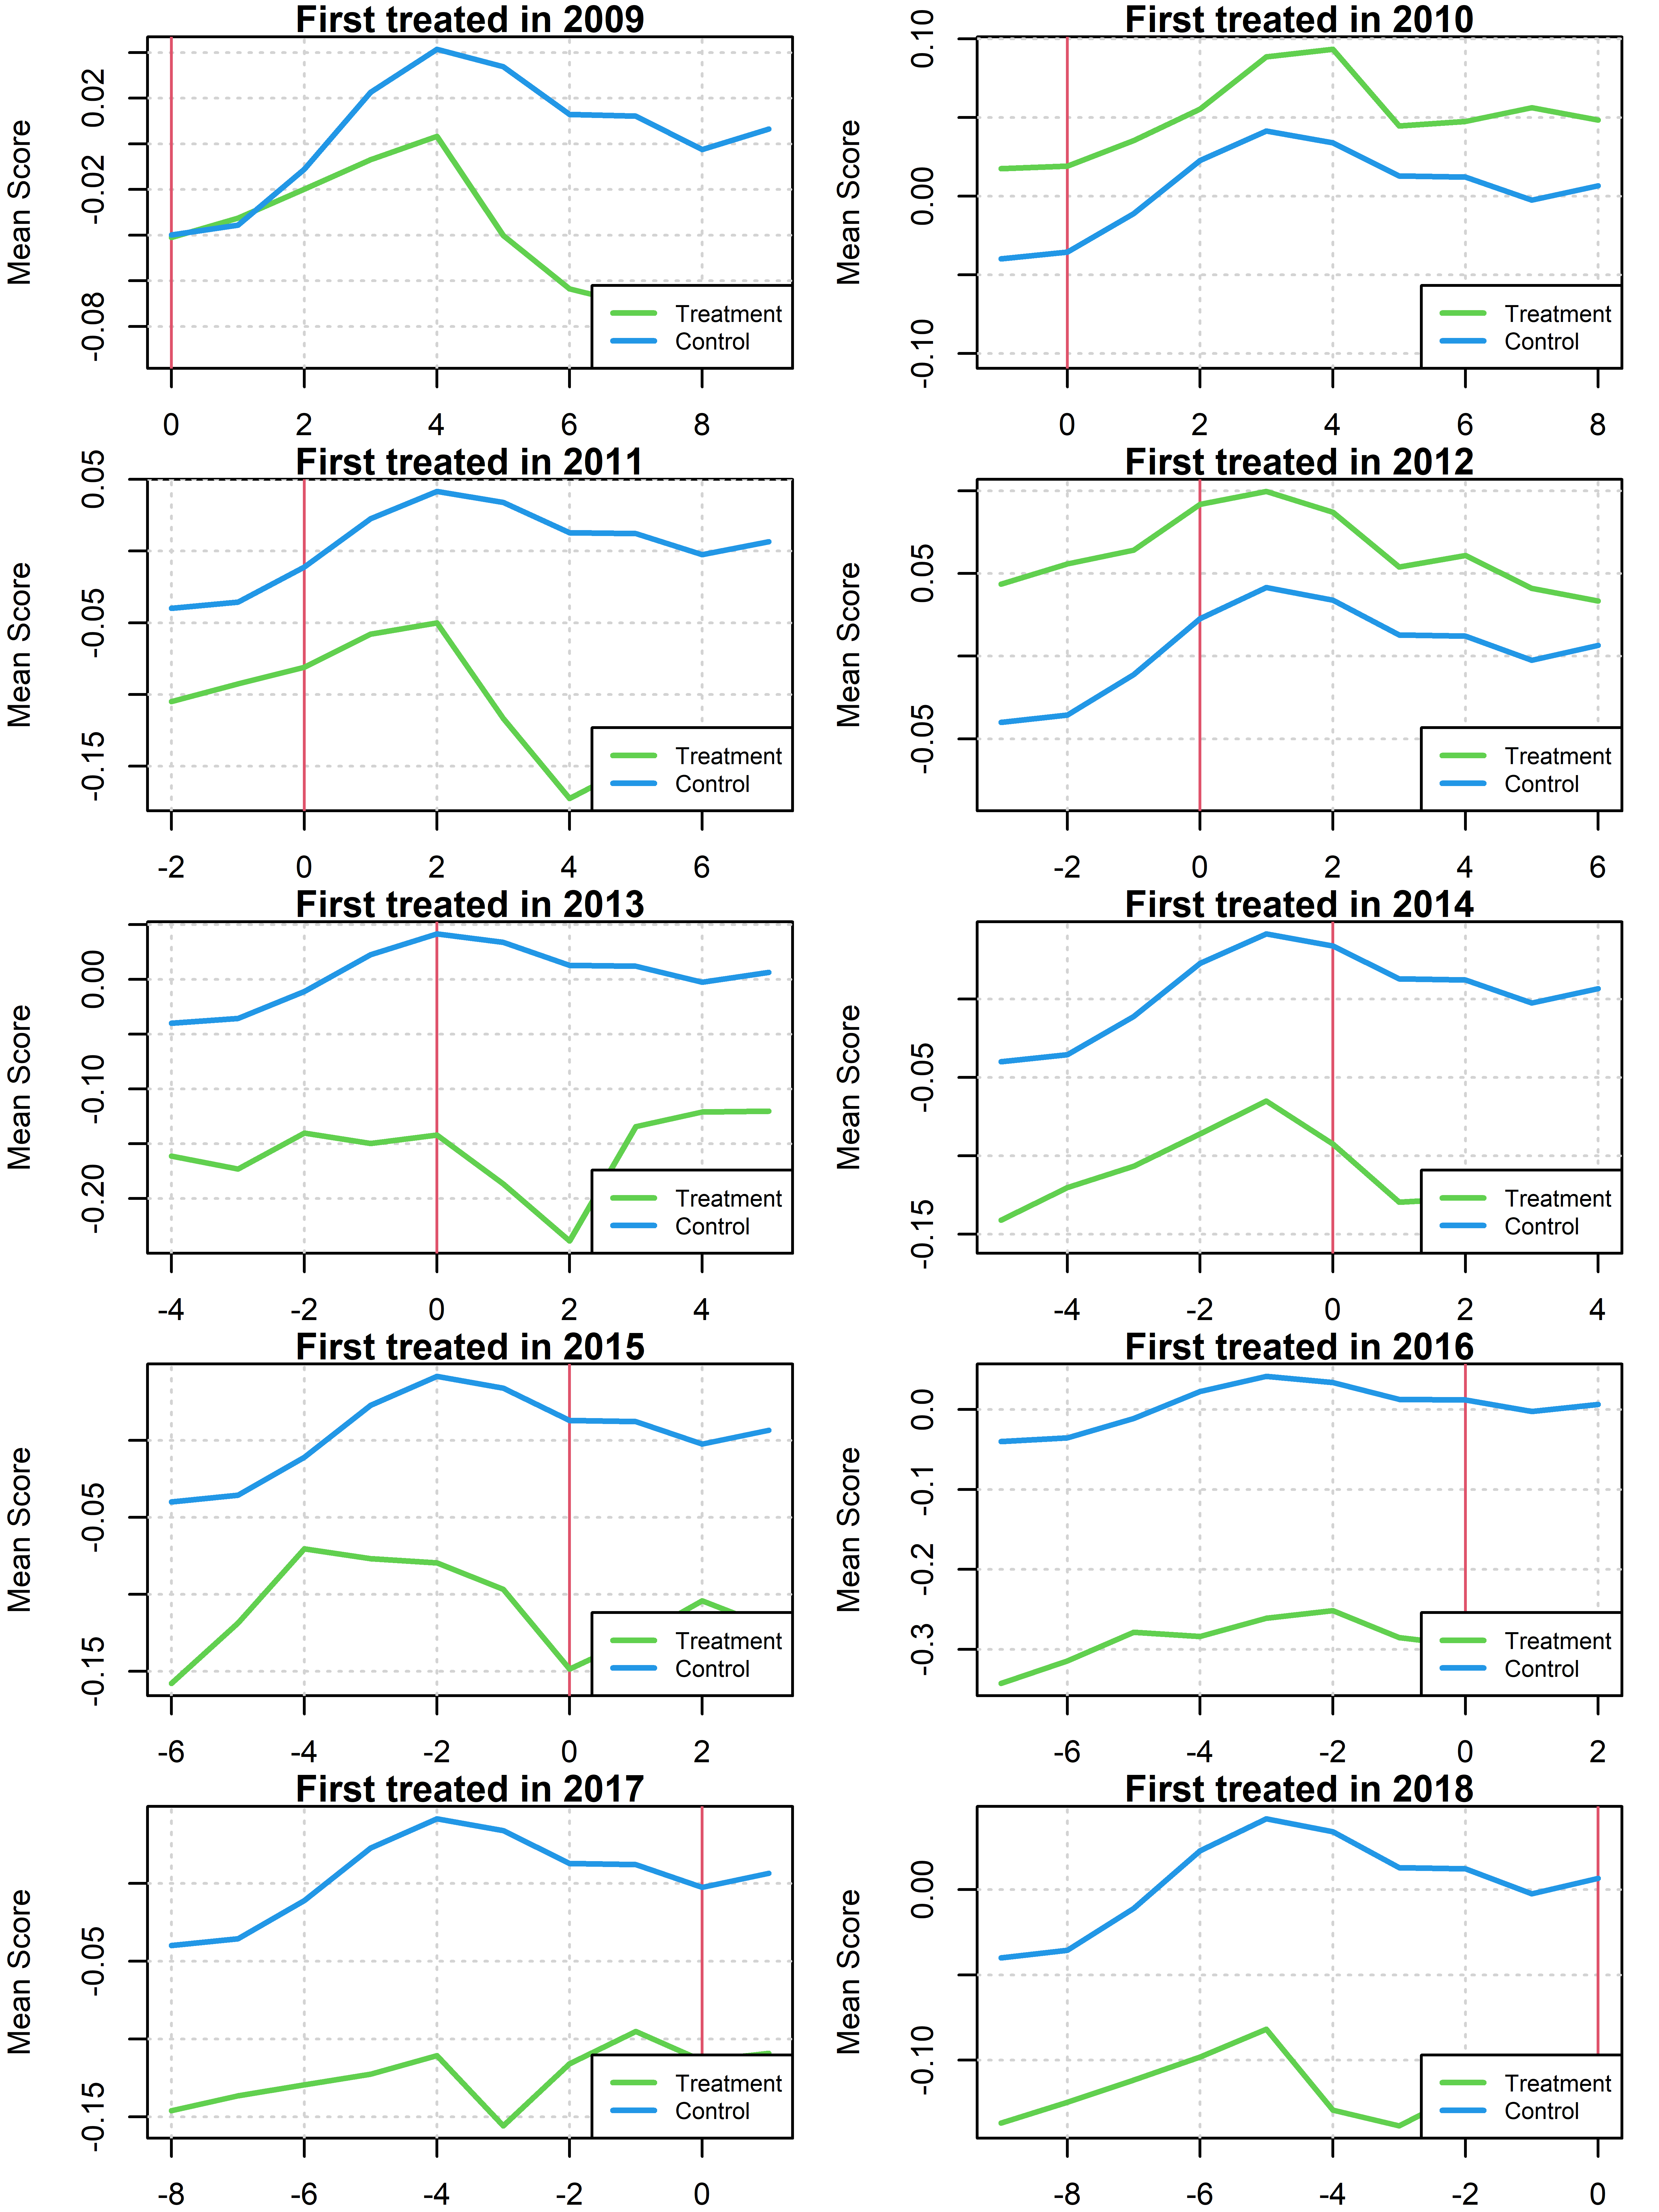
\includegraphics[scale=1]{"../Code & Data/ParTrendsPlotMathematics.png"}
	\caption{Pre trends for aggregated mean scores in mathematics}
	\label{PreTrendsMath}
\end{figure}

\begin{figure}[!h]
	\centering
	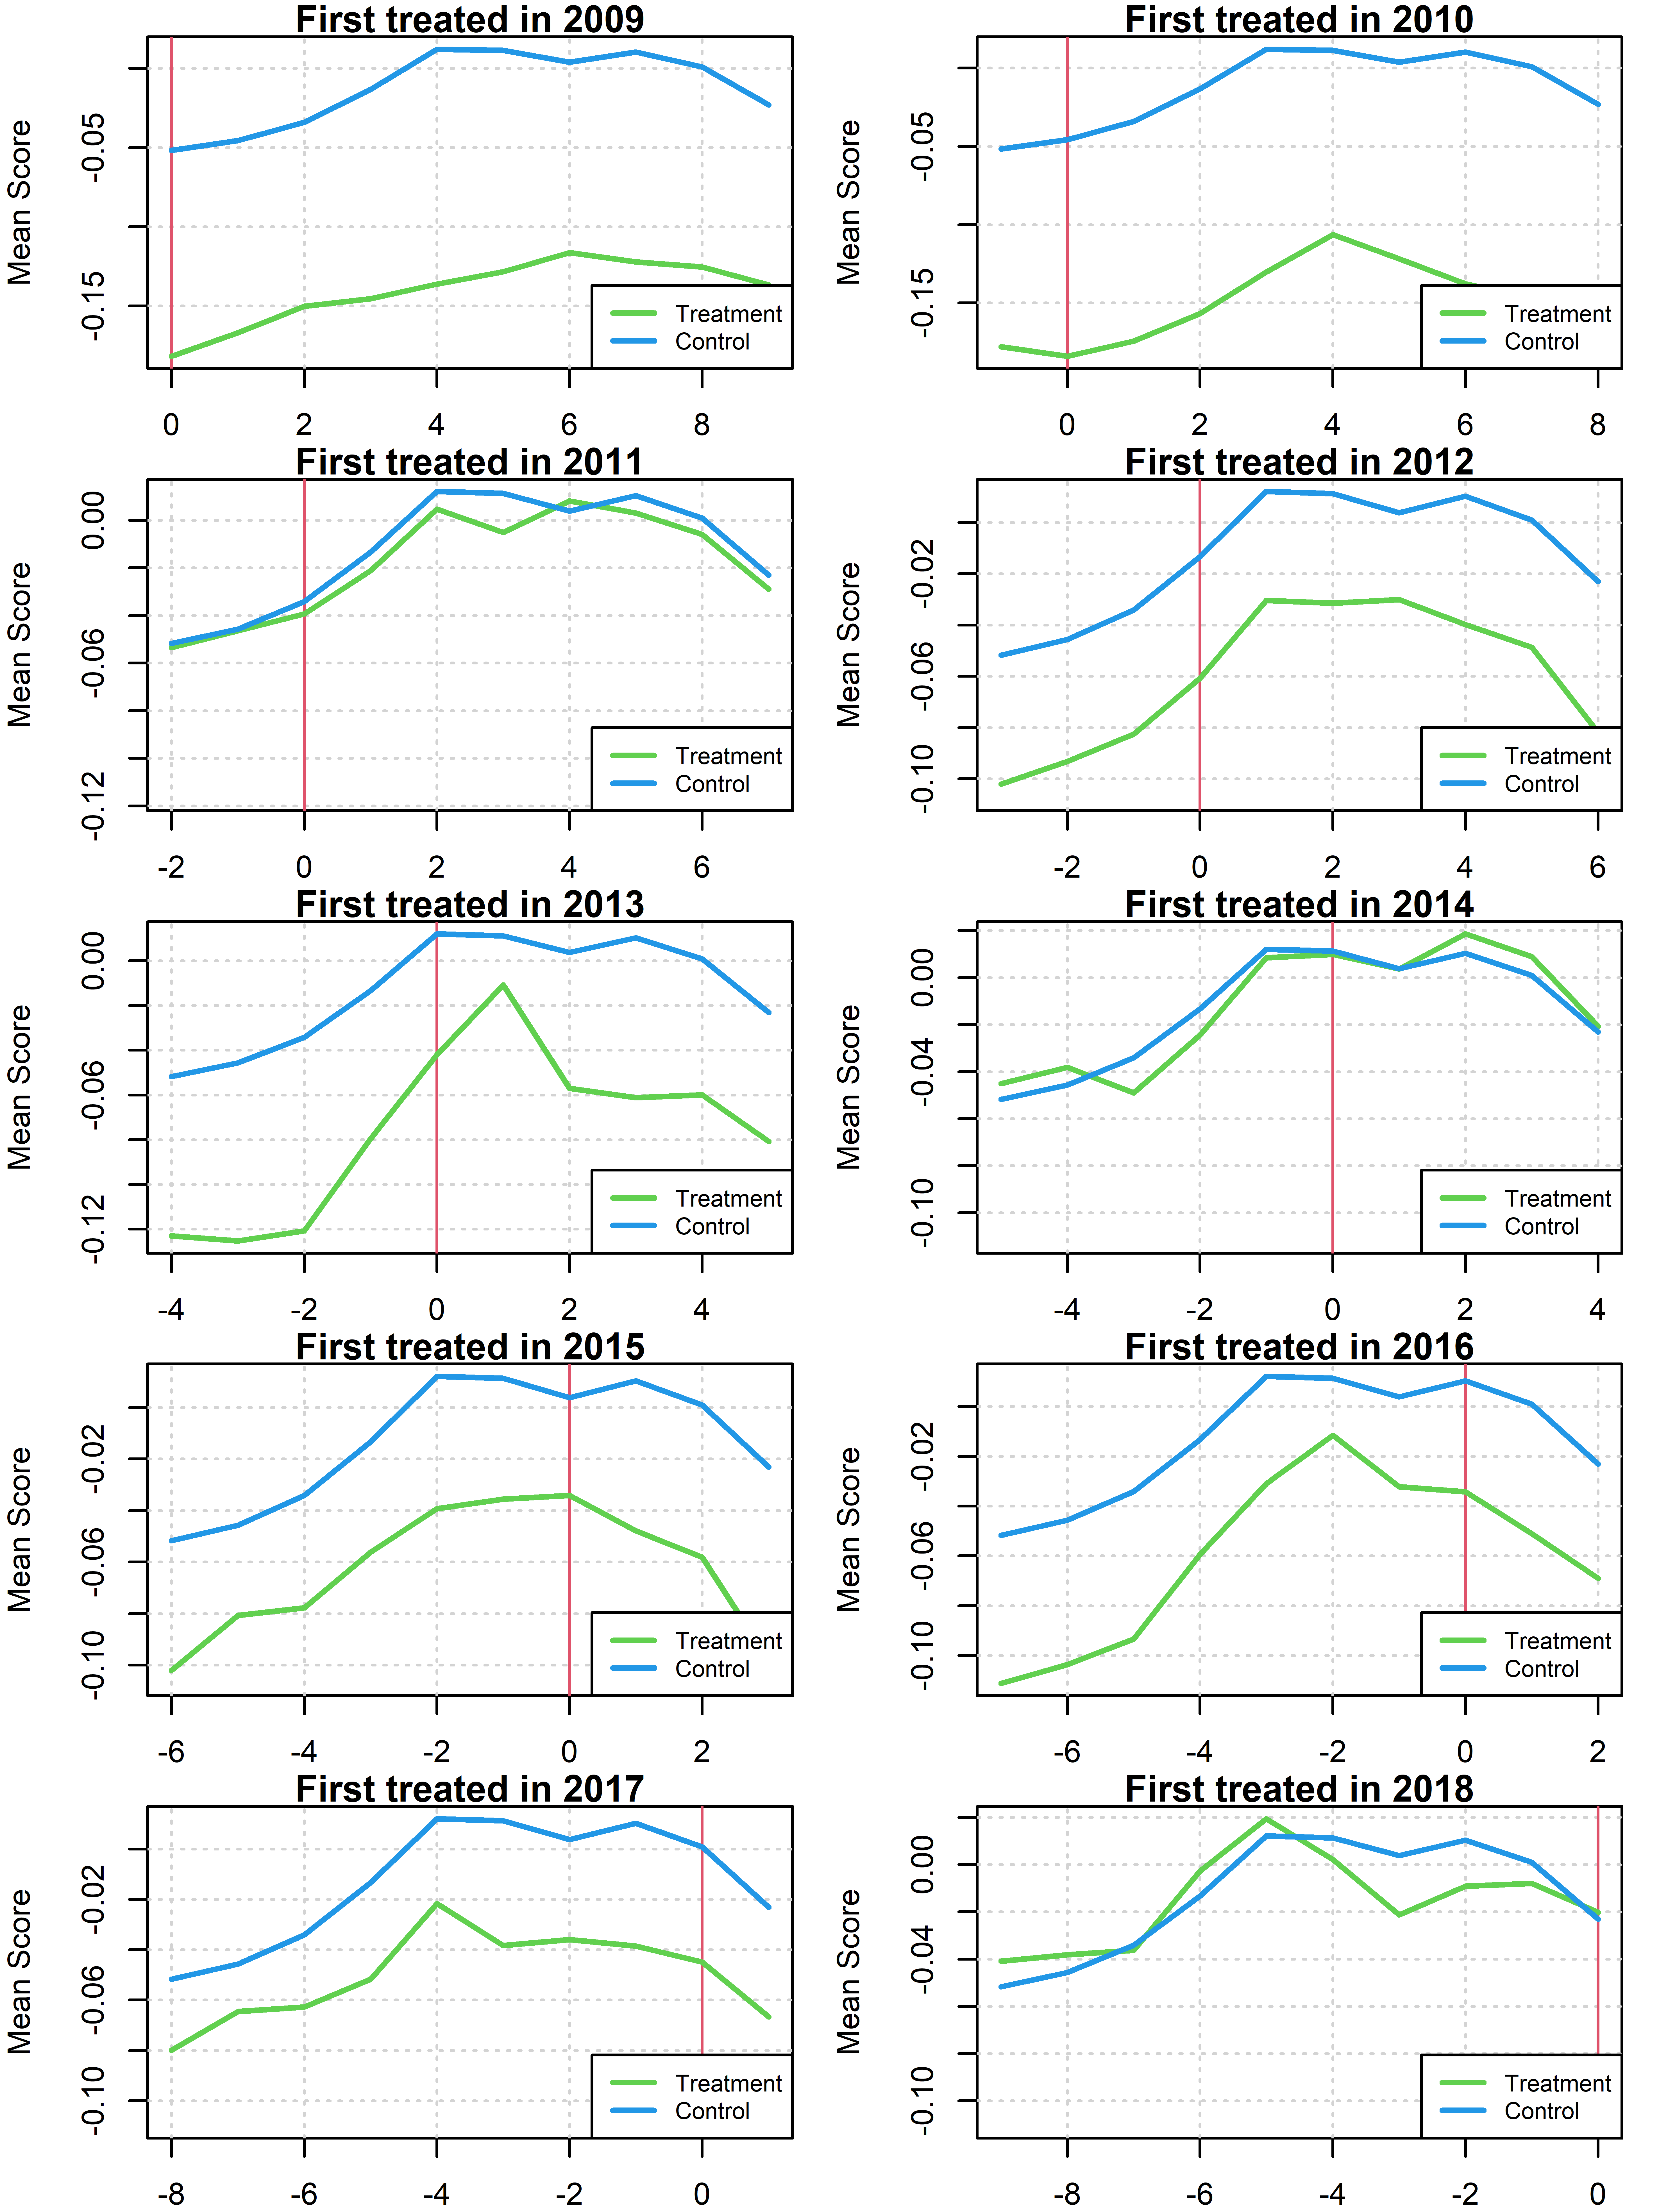
\includegraphics[scale=1]{"../Code & Data/ParTrendsPlotRLA.png"}
	\caption{Pre trends for aggregated mean scores in RLA}
	\label{PreTrendsRLA}
\end{figure}





% appendix

% bibliography
\bibliographystyle{apalike}
\bibliography{references}

\end{document}          



